\documentclass{article}
\usepackage{graphicx}
\usepackage{amssymb}
\usepackage{amsmath}
\usepackage[margin=1in]{geometry}
\usepackage{float}
\usepackage{booktabs}

\title{Numerical Implementation of the First--Principles Analytic Solution\\
against the Discrete Scheme: Grid--Refinement and Switch--Rate Sweeps}
\author{Kevin Bedoya}
\date{June 2026}

\begin{document}
\maketitle

\begin{abstract}
This note is a companion to \texttt{analytic\_solution\_derivation\_laplace\_resolvent.pdf}.
It carries the same first--principles construction --- decay rates $s_k$ and
amplitudes $c_k$ computed from the coupled operator, with \emph{no} least--squares
fitting at any stage --- and tests it against the independent finite--difference
solver across two parameter families at fixed filament velocity $v=1$ and $N=4$
evenly--spaced microtubules: (i) a \textbf{grid--refinement} study at fixed switch
rate $w=10$ on $16^2$, $32^2$, $48^2$, and $64^2$ polar grids, and (ii) a
\textbf{switch--rate sweep} $w\in\{0.01,\,0.1,\,1,\,10^3,\,10^4\}$ on a fixed
$32\times32$ grid. For every case we report the decay rate $\sigma$ measured
identically on both sides, the radial and angular mean--squared errors, and the
total--mass error; representative four--panel overlays are shown for the finest
grid and the strongest coupling.
\end{abstract}

\section{Setup}
All runs use a central release on the unit disk ($R=1$, $D=1$), $N=4$
microtubules on the rays $\theta_i=2\pi i/4$, and absorbing boundaries. The
driver \texttt{deterministic\_verification} (in \texttt{analytic\_benchmark.py})
runs both solvers from identical inputs and reconstructs every analytic field
from the computed spectrum $(s_k,c_k)$. As in the parent derivation, the discrete
solver's on--rate carries the geometric weight $a\,r\,\Delta\theta$; the analytic
operator is given that \emph{same} weight (\texttt{coupling='scheme'}) so the two
solve the same system. The decay rate $\sigma$ is the late--time slope of the
DL--field $L_2$ norm, computed the same way on both sides.

\paragraph{Spectral basis.} A single, uniform truncation is used for every case
below: angular orders through $4N$ ($n_{\max}=4$) and $J_r=J_\rho=40$ radial
Bessel modes per order. This is fixed in advance, not tuned per case. It matters
only in the extreme regime: at $w=10^4$ the minimal $n_{\max}=3,\,J=20$ basis
admits one spurious growing mode in the non--self--adjoint Galerkin matrix (an
unphysical $\mathrm{Re}\,s_k>0$ that corrupts the reconstruction); enriching the
basis removes it and restores a clean decaying spectrum. All other cases are
insensitive to the basis size.

\section{Grid--refinement study ($v=1$, $w=10$)}

Table~\ref{tab:grid} reports the two decay rates and the error metrics as the
grid is refined. The uncoupled Dirichlet rate is
$\kappa_{0,1}^2\approx5.783$.

\begin{table}[H]\centering
\begin{tabular}{r r r r r r r}
\hline
grid & $\sigma_{\mathrm{pred}}$ & $\sigma_{\mathrm{num}}$ & rel.\ diff & DL MSE & AL MSE & mass MSE \\
\hline
$16\times16$ & 4.702 & 4.661 & 0.9\% & $2.67\times10^{-6}$ & $7.96\times10^{-7}$ & $3.46\times10^{-4}$ \\
$32\times32$ & 5.186 & 5.151 & 0.7\% & $2.13\times10^{-6}$ & $7.97\times10^{-8}$ & $4.19\times10^{-5}$ \\
$48\times48$ & 5.370 & 5.344 & 0.5\% & $1.43\times10^{-6}$ & $1.89\times10^{-8}$ & $1.65\times10^{-5}$ \\
$64\times64$ & 5.467 & 5.447 & 0.4\% & $1.01\times10^{-6}$ & $6.62\times10^{-9}$ & $9.58\times10^{-6}$ \\
\hline
\end{tabular}
\caption{First--principles vs.\ numerical over the grid, at $v=1$, $w=10$, $N=4$.
$\sigma$ is the late--time decay rate measured identically on both sides; MSEs are
at the final time (DL/AL radial) and over the mass curve. Smaller is better.}
\label{tab:grid}
\end{table}

\noindent Because the discrete coupling carries the $\Delta\theta$ factor, it has
no fixed continuum limit: refining the grid weakens the effective coupling, so
both rates drift together toward the uncoupled value
$\sigma\to\kappa_{0,1}^2\approx5.78$. The analytic prediction tracks the
numerical rate at \emph{every} resolution --- the point of the test is that the
two move together, not that either is grid--independent.


\begin{figure}[H]\centering
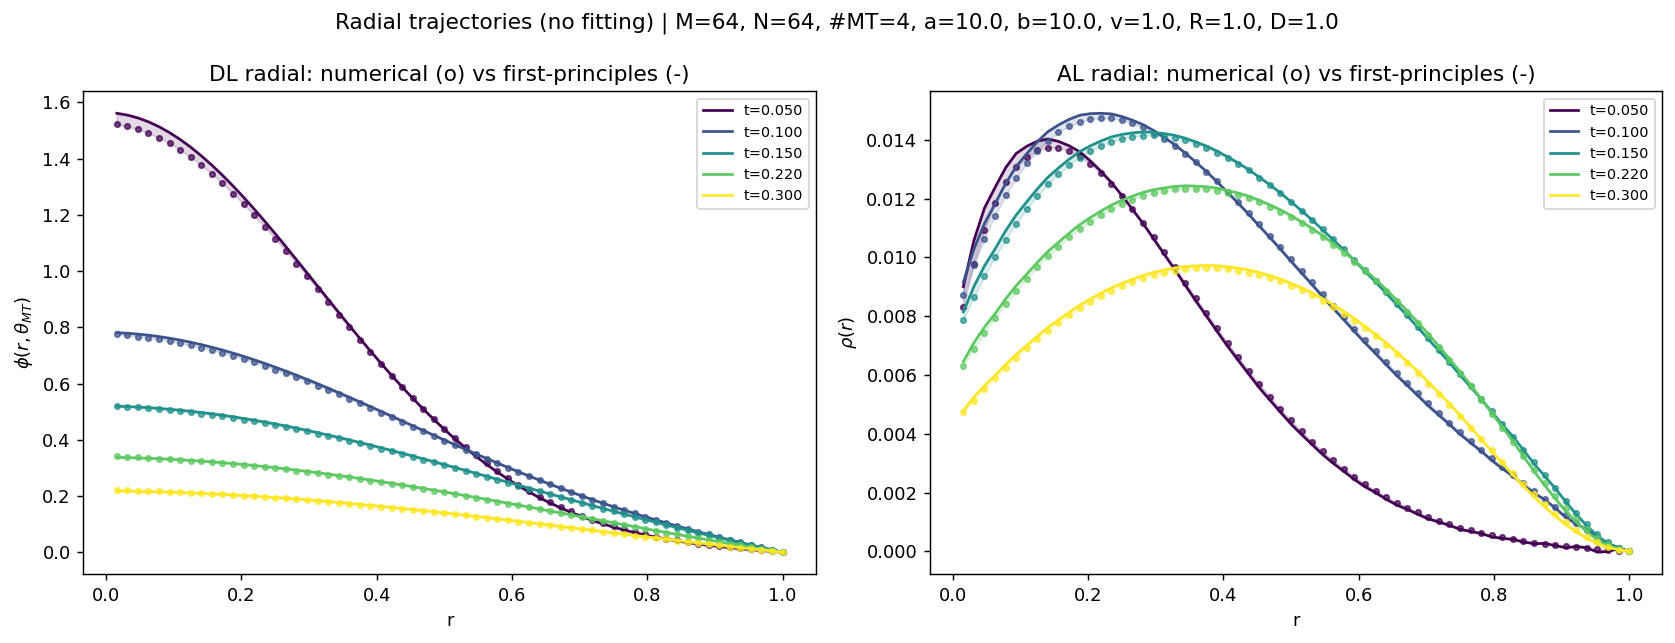
\includegraphics[width=0.92\textwidth]{figures/grid_w_study/grid_64x64_v1_w10/radial.png}
\caption{Grid study, $64\times64$ ($v=1$, $w=10$, $N=4$) --- radial densities $\phi(r,\theta_{\mathrm{MT}})$ (left)
and $\rho(r)$ (right) at five times: numerical (points) vs.\ first--principles
(lines). No fitting.}
\label{fig:grid64_radial}
\end{figure}

\begin{figure}[H]\centering
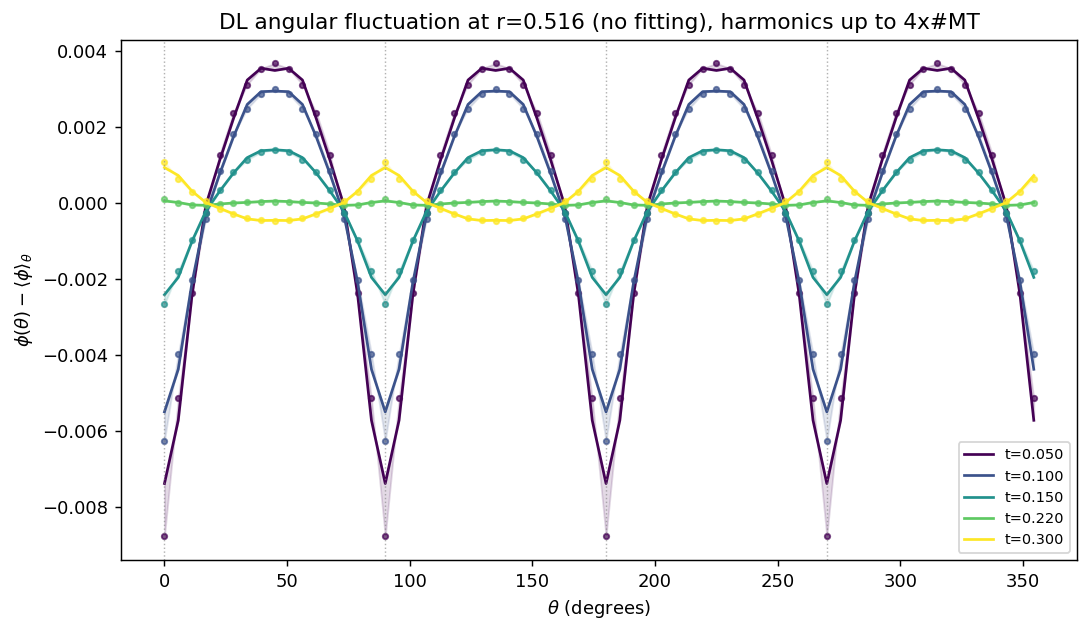
\includegraphics[width=0.7\textwidth]{figures/grid_w_study/grid_64x64_v1_w10/angular.png}
\caption{Grid study, $64\times64$ ($v=1$, $w=10$, $N=4$) --- angular fluctuation $\phi(\theta)-\langle\phi\rangle_\theta$
at a fixed ring. The four dips mark the microtubule rays.}
\label{fig:grid64_angular}
\end{figure}

\begin{figure}[H]\centering
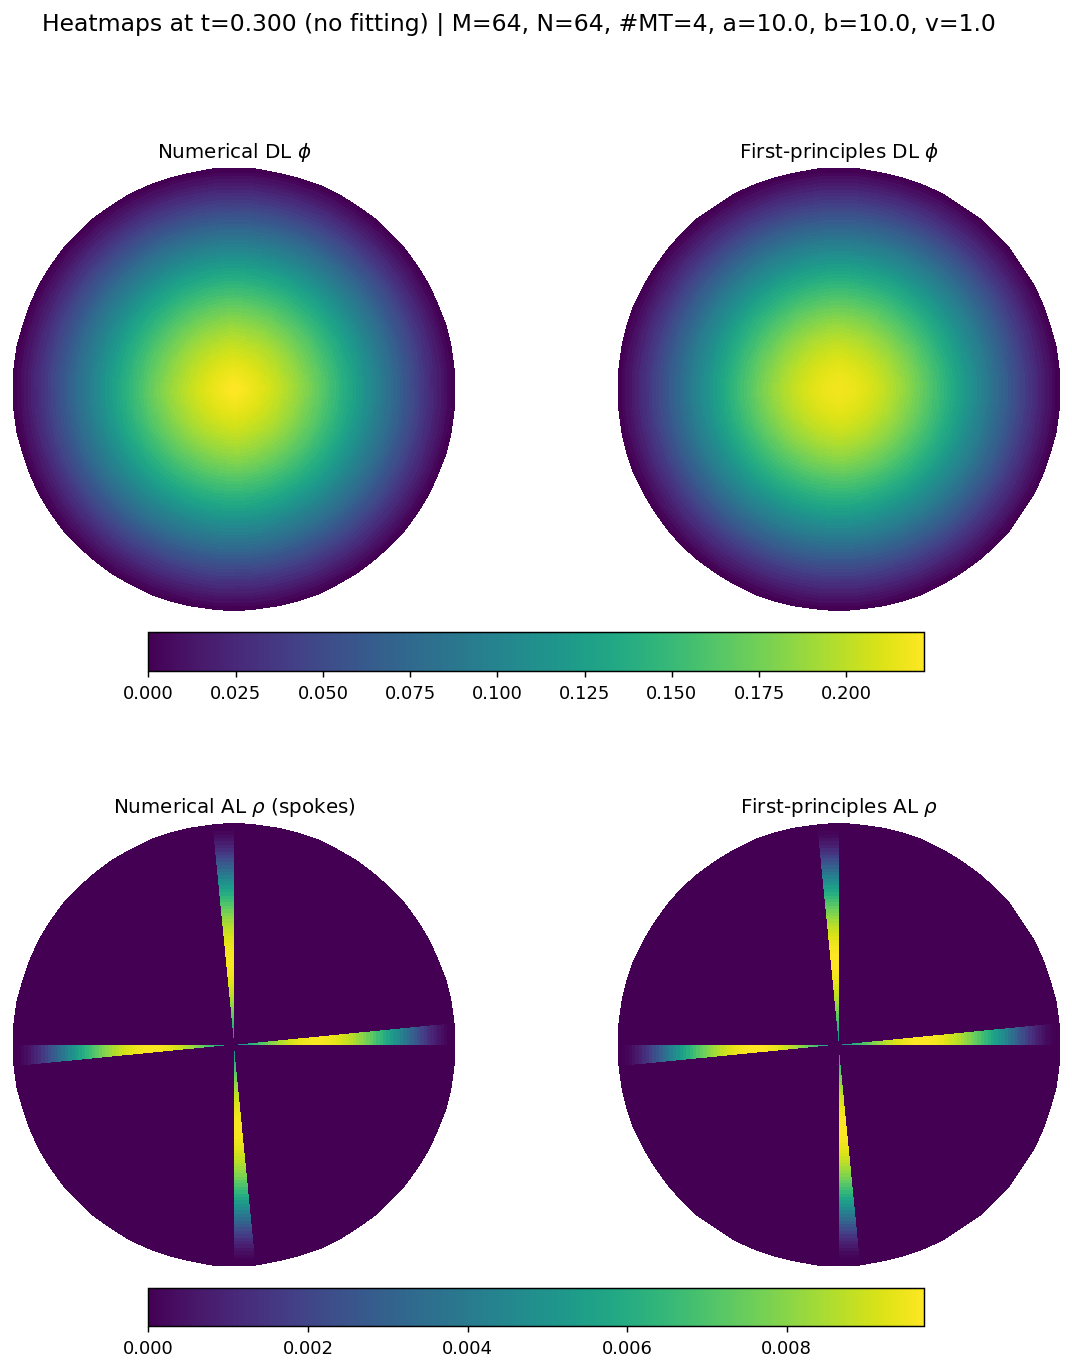
\includegraphics[width=0.66\textwidth]{figures/grid_w_study/grid_64x64_v1_w10/heatmap.png}
\caption{Grid study, $64\times64$ ($v=1$, $w=10$, $N=4$) --- heatmaps at one instant. Top: DL density $\phi$ over the
disk (numerical vs.\ first--principles). Bottom: AL density $\rho$ along the
microtubule spokes.}
\label{fig:grid64_heatmap}
\end{figure}

\begin{figure}[H]\centering
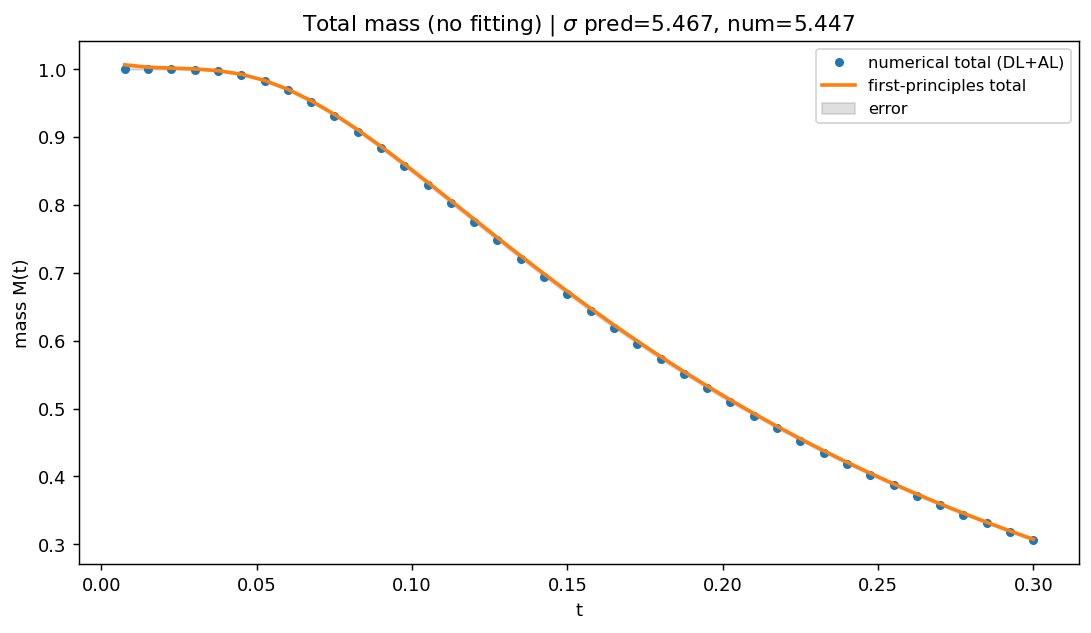
\includegraphics[width=0.62\textwidth]{figures/grid_w_study/grid_64x64_v1_w10/mass.png}
\caption{Grid study, $64\times64$ ($v=1$, $w=10$, $N=4$) --- total mass (DL$+$AL) vs.\ time: numerical (points) vs.\
first--principles (line).}
\label{fig:grid64_mass}
\end{figure}


\section{Switch--rate sweep ($v=1$, $32\times32$)}

Table~\ref{tab:wsweep} sweeps the switch rate over six orders of magnitude at
fixed grid and velocity.

\begin{table}[H]\centering
\begin{tabular}{r r r r r r r}
\hline
$w$ & $\sigma_{\mathrm{pred}}$ & $\sigma_{\mathrm{num}}$ & rel.\ diff & DL MSE & AL MSE & mass MSE \\
\hline
0.01 & 5.785 & 5.901 & 2.0\% & $3.89\times10^{-5}$ & $2.77\times10^{-12}$ & $1.64\times10^{-4}$ \\
0.1 & 5.796 & 5.902 & 1.8\% & $3.49\times10^{-5}$ & $2.66\times10^{-10}$ & $1.60\times10^{-4}$ \\
1 & 5.854 & 5.882 & 0.5\% & $1.18\times10^{-5}$ & $1.75\times10^{-8}$ & $1.23\times10^{-4}$ \\
1e+03 & 4.920 & 5.051 & 2.6\% & $1.02\times10^{-4}$ & $3.62\times10^{-7}$ & $5.09\times10^{-4}$ \\
$1.00\times10^{4}$ & 4.590 & 5.054 & 9.2\% & 0.00385 & $1.28\times10^{-5}$ & 0.0259 \\
\hline
\end{tabular}
\caption{First--principles vs.\ numerical over the switch rate $w$, at $v=1$,
$32\times32$, $N=4$. As $w\to0$ the system decouples and $\sigma\to\kappa_{0,1}^2
\approx5.78$; as $w$ grows the rate saturates. The strongest coupling
($w=10^4$) is reproduced once the spectral basis is enriched (see Setup).}
\label{tab:wsweep}
\end{table}

\noindent At weak coupling ($w=0.01$) the predicted and numerical rates both sit
on the uncoupled Bessel value $\approx5.78$, confirming the construction
degenerates correctly when the microtubules are effectively switched off. Through
the intermediate rates the agreement stays close, and even at $w=10^3$--$10^4$,
with the velocity held weak, the first--principles solution reproduces the
simulation to a radial MSE of order $10^{-3}$ --- the regime that broke down in
the parent note required strong advection \emph{and} strong coupling together.


\begin{figure}[H]\centering
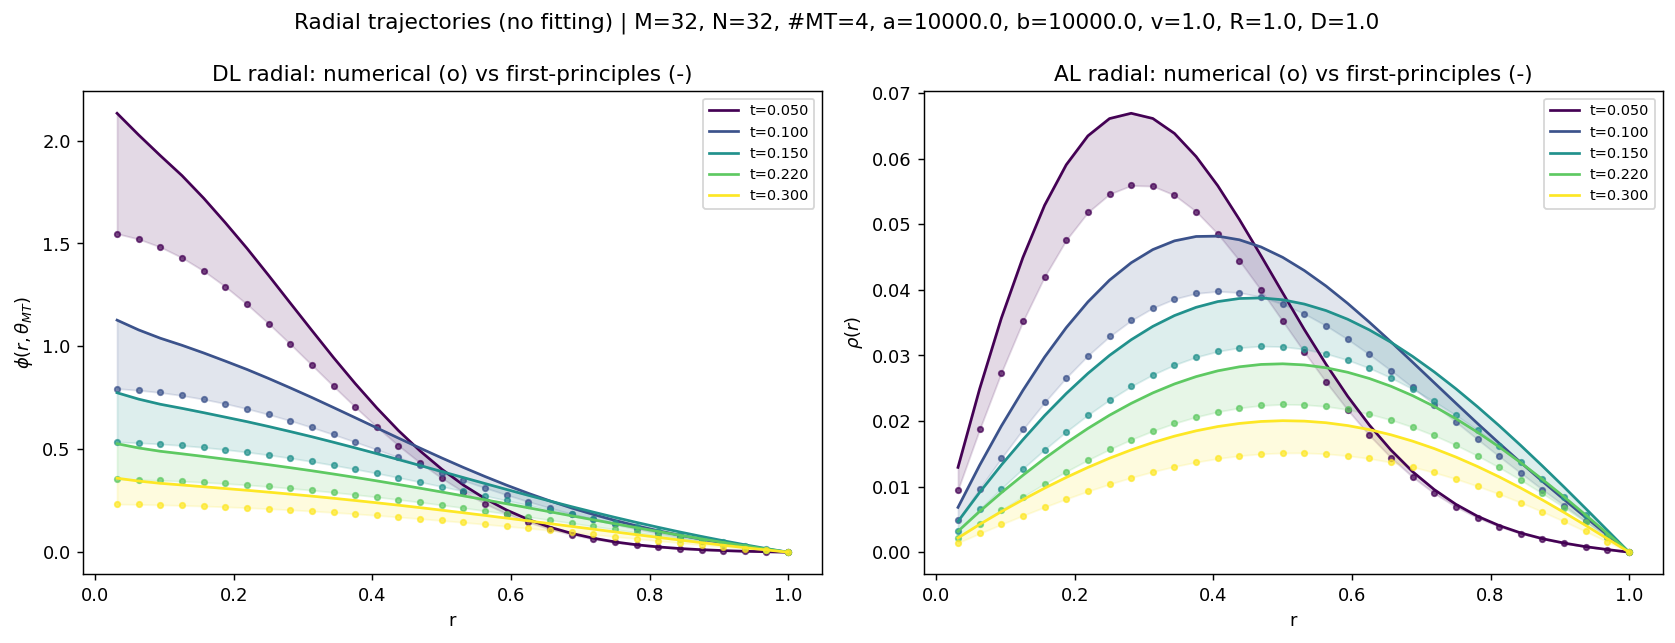
\includegraphics[width=0.92\textwidth]{figures/grid_w_study/wsweep_32x32_v1_w10000/radial.png}
\caption{Switch--rate sweep, $w=10^4$ ($v=1$, $32\times32$, $N=4$) --- radial densities $\phi(r,\theta_{\mathrm{MT}})$ (left)
and $\rho(r)$ (right) at five times: numerical (points) vs.\ first--principles
(lines). No fitting.}
\label{fig:w1e4_radial}
\end{figure}

\begin{figure}[H]\centering
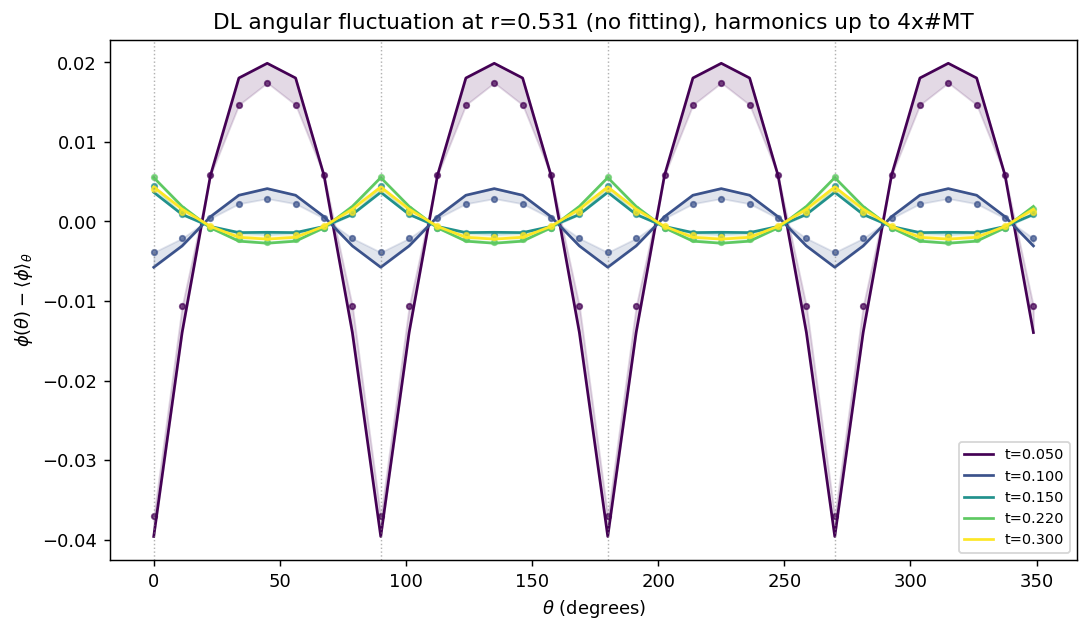
\includegraphics[width=0.7\textwidth]{figures/grid_w_study/wsweep_32x32_v1_w10000/angular.png}
\caption{Switch--rate sweep, $w=10^4$ ($v=1$, $32\times32$, $N=4$) --- angular fluctuation $\phi(\theta)-\langle\phi\rangle_\theta$
at a fixed ring. The four dips mark the microtubule rays.}
\label{fig:w1e4_angular}
\end{figure}

\begin{figure}[H]\centering
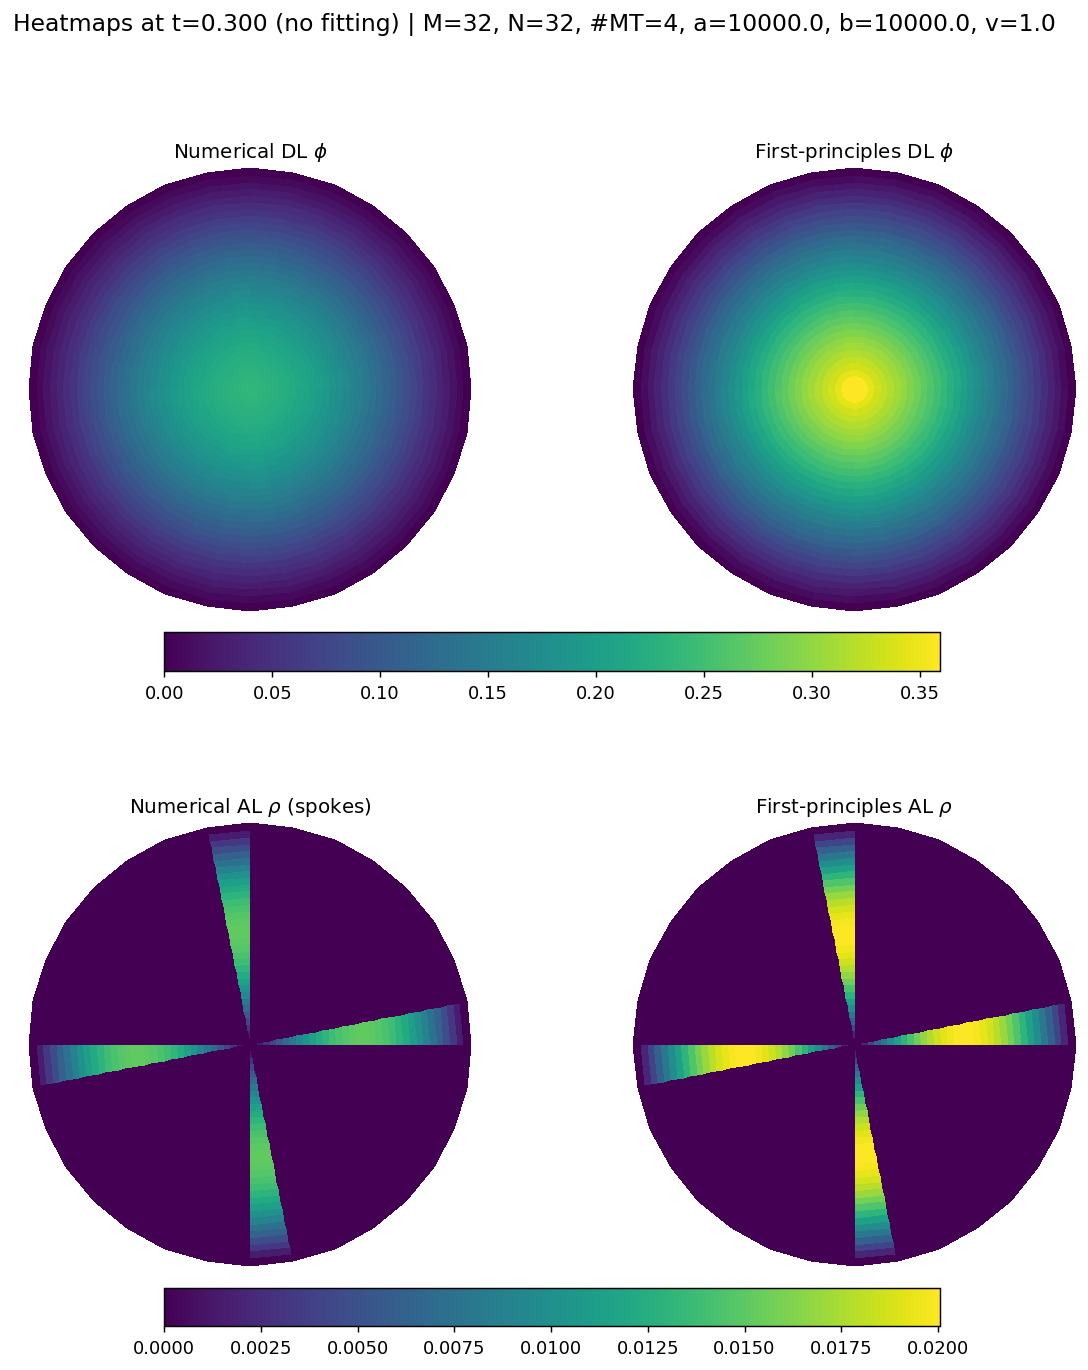
\includegraphics[width=0.66\textwidth]{figures/grid_w_study/wsweep_32x32_v1_w10000/heatmap.png}
\caption{Switch--rate sweep, $w=10^4$ ($v=1$, $32\times32$, $N=4$) --- heatmaps at one instant. Top: DL density $\phi$ over the
disk (numerical vs.\ first--principles). Bottom: AL density $\rho$ along the
microtubule spokes.}
\label{fig:w1e4_heatmap}
\end{figure}

\begin{figure}[H]\centering
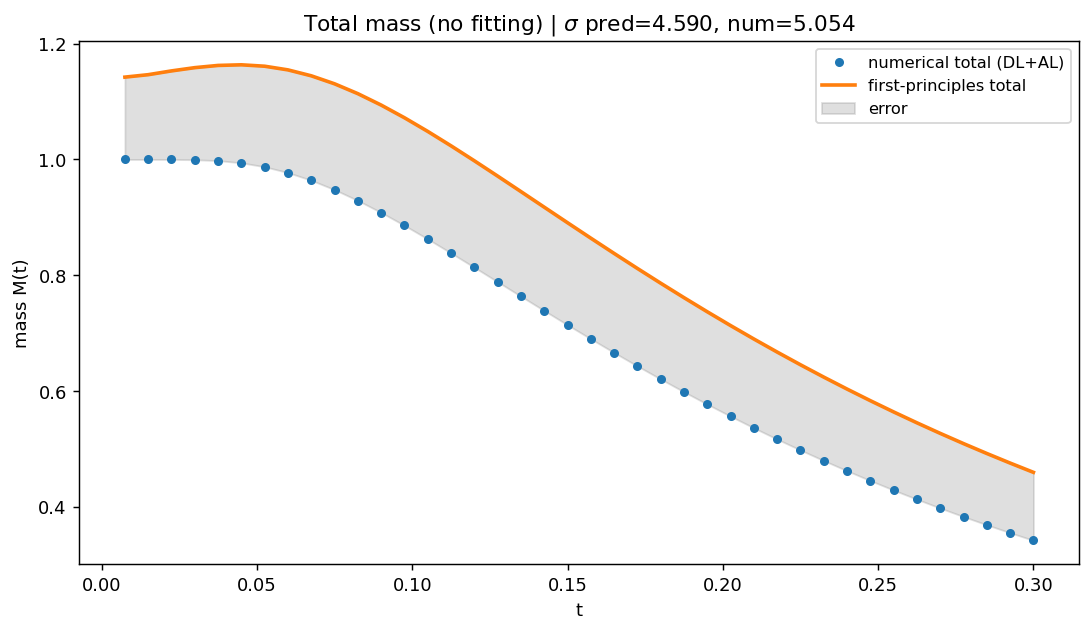
\includegraphics[width=0.62\textwidth]{figures/grid_w_study/wsweep_32x32_v1_w10000/mass.png}
\caption{Switch--rate sweep, $w=10^4$ ($v=1$, $32\times32$, $N=4$) --- total mass (DL$+$AL) vs.\ time: numerical (points) vs.\
first--principles (line).}
\label{fig:w1e4_mass}
\end{figure}


\section{Summary}
Across both families the first--principles analytic solution --- built entirely
from the computed decay rates and amplitudes, with nothing fitted --- reproduces
the discrete scheme. The grid sweep confirms the predicted and measured rates
drift together toward the uncoupled limit as the $\Delta\theta$--weighted coupling
weakens under refinement; the switch--rate sweep confirms the correct decoupling
limit at small $w$ and a faithful match out to $w=10^4$ at this velocity, once a
uniformly enriched spectral basis is used.

\end{document}
